%% Elsevier elsarticle template (num style) adapted for the journal manuscript.
%% The manuscript keeps one sentence per line in the source.

\documentclass[preprint,12pt]{elsarticle}

\usepackage{amssymb}
\usepackage{amsmath}
\usepackage{lineno}
\usepackage{xcolor}
\usepackage{array}
\usepackage{multirow}
\usepackage{pifont}
\usepackage{adjustbox}
\usepackage{booktabs}
\usepackage{graphicx}
\usepackage{url}
\usepackage{placeins}

\setlength{\emergencystretch}{2em}
\setlength{\abovecaptionskip}{8pt plus 2pt minus 1pt}
\setlength{\belowcaptionskip}{8pt plus 2pt minus 1pt}
\setlength{\textfloatsep}{16pt plus 3pt minus 2pt}
\setlength{\floatsep}{14pt plus 3pt minus 2pt}
\setlength{\intextsep}{14pt plus 3pt minus 2pt}

\newcommand{\cmark}{\ding{51}}
\newcommand{\xmark}{\ding{55}}
\newcommand{\pmark}{\textcolor{orange}{$\sim$}}
\newcommand{\rev}[1]{\textcolor{blue}{#1}}
\newcommand{\del}[1]{\textcolor{red}{#1}}

\journal{Information Fusion}

\begin{document}

\begin{frontmatter}

\title{Cross-Modal Generative Alignment for Document, Chart, and Image
Reasoning with Explanation-Aware Vision--Language Models}

\author[label1]{Komron Valijonov}
\author[label1,label2]{Raja Hashim Ali}

\affiliation[label1]{organization={Department of Business, University of Europe for Applied Sciences},
            addressline={Think Campus, Konrad-Zuse-Ring 11},
            city={Potsdam},
            postcode={14469},
            state={Brandenburg},
            country={Germany}}

\affiliation[label2]{organization={Department of Artificial Intelligence, Ghulam Ishaq Khan Institute of Engineering Sciences and Technology},
            city={Topi},
            postcode={23460},
            country={Pakistan}}

\begin{abstract}
A vision-language model (VLM) is able to read a chart, document, scanned form, or natural image and answer questions about it. 
But how do we know if the answer is actually derived from the image itself, rather than being a lucky guess on a question based on the model's remembered language patterns?
The correctness of the answer itself is not enough if the reasoning for that answer is not grounded in the visual evidence of the image.
Charts and documents are a good example of this problem, because to answer the question correctly, the model has to actually ground its reasoning on specific parts of the image,
making it easier to spot when the model is looking at the wrong thing. Although recent work has made progress on this issues,
there was no isolation of the training objective as the main variable, with all other factors such as the model, the data, and the budget held constant.
Contrastive, generative, and explanation-based methods have all been proposed, but they have not been directly compared under the same conditions,
so it is not clear what the objective itself contributed to the final performance. 
In this paper, we keep the pipeline fixed and change only the training signal, so we can see what the objective does to answer accuracy, explanation quality, 
and evidence sensitivity when the model, the data, and the compute budget are all held steady.
We compare five settings head to head rather than treating them as unrelated systems: BLIP-2 generative fine-tuning, BLIP-2 contrastive-enhanced fine-tuning,
Qwen2-VL under answer-only, rationale-generative, and explanation-aware supervision.
All the runs use the same resource-constrained single-seed protocol, and the same evaluation code as much as possible,
across ScienceQA, A-OKVQA, ChartQA, DocVQA, and a VQAv2 subset.
The picture that emerges is mixed. On ScienceQA, Qwen2-VL-2B reaches 0.800 accuracy with answer-only supervision,
0.780 in both rationale-generative and length-aware explanation control settings, and 0.765 with fixed-alpha explanation-aware training.
On A-OKVQA, the same model reaches 0.830 with answer-only supervision, 0.790 in both rationale-generative and length-aware explanation control training,
and 0.795 with fixed-alpha explanation-aware training.
ChartQA, DocVQA, and the VQAv2 subset have no gold rationales, so those runs fall back to answer-only controls;
they lift the native headline metrics, but they do not test rationale supervision at all.
BLIP-2 barely moves: the contrastive objective gives a small gain compared to the generative one on ScienceQA 0.480 vs 0.475,
but the retrieval diagnostic stays near frozen and random controls in both cases.
Scale is the exception. With a fixed explanation-aware objective on ScienceQA, Qwen2-VL-7B reaches 0.885 while the 2B version reaches 0.765.
The masking analysis tells us whether the model relies on the image, not whether its explanation is faithful.
Overall, the results do not show a clear win for explanation-aware training.
The rationale supervision can help on a single-GPU budget, but the gain is easy to mis-credit to scale or tuning.
Hence, it only stands up when answer-only controls, objective balance, model scale, transfer and evidence sensitivity are each reported separately. 
\end{abstract}

\begin{graphicalabstract}
\centering
\includegraphics[width=\linewidth]{Figures/icons/Abstract_L}
\end{graphicalabstract}

\begin{highlights}
\item The study separates zero-shot, answer-only, rationale-generative, explanation-aware, and BLIP-2 contrastive-enhanced controls under one capped single-GPU protocol.
\item On the rationale-bearing datasets, answer-only controls are strong; explanation-aware training is competitive but not automatically best.
\item BLIP-2 contrastive-enhanced fine-tuning gives only a small ScienceQA gain over BLIP-2 generative fine-tuning, and the retrieval diagnostic stays near frozen and random controls.
\item Evidence-masking drift is reported as evidence sensitivity, so answer gains, rationale quality, and grounding claims are kept separate.
\end{highlights}

\begin{keyword}
vision--language models \sep cross-modal alignment \sep explanation-aware training \sep chart and document understanding \sep faithfulness \sep parameter-efficient fine-tuning
\end{keyword}

\end{frontmatter}

\linenumbers

\section{Introduction}

Vision--language models (VLMs) have turned into a default tool for reading images, documents, and charts and answering questions about them.
The task looks simple from the outside: you hand the model an image and a question, and it should hand back an answer the image actually supports.
What counts as evidence, though, depends entirely on the picture.
In a document it might be buried in a line of body text, in the table structure, or in one small stamped region of a scanned page.
In a chart it might live in an axis label, the relative height of two bars, a colour, or a trend nobody ever wrote down in words.
In science and commonsense visual question answering (VQA), it is often not in the image at all, and the model has to fold in background knowledge it already carries.
Across every one of these, a confident, correct-looking answer is worth little if the reasoning underneath it is not grounded in the image.
Models are very good at sounding right while looking at the wrong thing.
So we study the answer and the explanation together, not one or the other.

Underneath all of it sits one idea: cross-modal alignment, the job of wiring the visual signal into the language model so the two actually talk.
How well that wiring works turns out to hinge on a long list of choices, namely visual resolution, data mixture, connector design, instruction tuning, and the adaptation method~\cite{laurencon2024whatmatters,zhang2025mm15,deitke2025molmo}.
Open model families help, because backbones such as Qwen2-VL, BLIP-2, and LLaVA-OneVision are strong out of the box yet still adaptable on an academic budget~\cite{wang2024qwen2vl,li2023blip2,li2025llavaonevision}.
They are not enough on their own, though.
Recent document and chart work keeps showing that general visual instruction following falls short on text-heavy, structured images~\cite{fu2025textrichsurvey,wang2024docllm,masry2024chartinstruct,masry2025chartgemma}.
There is a budget reality too.
Most students and small labs cannot fully fine-tune a large multimodal model, full stop.
Low-rank methods such as DoRA (weight-decomposed low-rank adaptation) make it realistic to touch only a sliver of the parameters while the base model stays frozen or quantised~\cite{liu2024dora}.
We take the same route, using low-rank adaptation (LoRA) and its quantised variant (QLoRA) instead of full-model fine-tuning~\cite{hu2022lora,dettmers2023qlora}.
The point is never to top a leaderboard; it is to watch what changes when the alignment objective changes and the budget stays real.

\subsection{Gap Analysis}
The gap is isolation.
A typical paper swaps the model, the data, the training size, and the objective in one move, reports a higher number, and credits the objective.
But you cannot actually tell.
Maybe the objective helped; maybe the model was simply bigger, or saw cleaner data.
Each objective also carries its own blind spot.
Contrastive learning is excellent at matching an image to its caption, yet it never directly teaches the model to write an answer or an explanation.
Generative learning trains that writing directly, but fluent text is no proof that the pixels were ever consulted.
Explanation-aware training goes a step further and supervises the reasoning itself, which is the appealing part; it is also how a model learns to produce a tidy rationale after the fact, decoration rather than cause.
And most of the hallucination and faithfulness literature still lives on natural images.
Documents and charts get less attention, even though their evidence is more structured and far easier to inspect, which is exactly what makes them a good stress test.
We close that gap by changing the alignment objective and holding everything else as steady as we can.

\subsection{Research Questions}
The main question is: how should a resource-constrained vision--language model be aligned when the goal is both accurate and faithful visual reasoning?
The following research questions make that question measurable.

\begin{enumerate}
    \item RQ1: How have vision--language alignment methods evolved for grounded visual reasoning and explanation generation?
    \item RQ2: How does BLIP-2 generative fine-tuning compare with BLIP-2 contrastive-enhanced fine-tuning on visual reasoning?
    \item RQ3: Does explanation-aware fine-tuning improve answer accuracy and explanation quality on datasets with gold rationales?
    \item RQ4: How does the same fine-tuning framework perform across document, chart, science, commonsense, and natural-image domains?
    \item RQ5: How sensitive are the model's answers to visual evidence under image-masking perturbations?
    \item RQ6: How does the selected explanation-aware QLoRA setup scale from Qwen2-VL-2B to Qwen2-VL-7B?
    \item RQ7: How well do fine-tuned adapters transfer across visual domains and prompt formats?
\end{enumerate}

\subsection{Problem Statement}
The problem is cross-modal alignment on the hardware most people actually have: a single GPU.
Starting from a pretrained vision--language model, we ask what the objective does to three things at once, namely answer accuracy, explanation quality, and how much the model leans on the image.
The backbone, the data format, the optimiser, and the evaluation procedure are pinned down wherever we can pin them.
Inside each comparison, only the training signal moves.
The BLIP-2 pair reuses one Q-Former training setup; the Qwen2-VL generative and explanation-aware runs reuse one QLoRA setup.
That is what keeps the study tractable instead of ballooning into a full-model fine-tuning project.
We are not optimising one benchmark score.
The question is narrower and more useful: does the objective move the model in a direction that matters for trustworthy reasoning?
A fluent explanation with no visual support is a failure here, even when the final answer happens to be right.

\subsection{Novelty of this study}
The contribution is the control, not a new architecture.
Rather than line up unrelated models or recipes against each other, we vary the objective and keep the surrounding setup as close to identical as the budget allows.
Faithfulness on structured inputs is treated as a first-class result here, not a couple of cherry-picked figures parked in the discussion.
Concretely, the paper contributes the following:

\begin{itemize}
    \item A single comparison that puts zero-shot, answer-only, BLIP-2 generative, BLIP-2 contrastive-enhanced, Qwen2-VL rationale-generative, and Qwen2-VL explanation-aware alignment under the same data and optimisation constraints.
    \item Evaluation along three separate axes, namely answer quality, explanation quality, and evidence sensitivity, across document, chart, science, commonsense, and natural-image tasks.
    \item A generate-then-score protocol for multiple-choice reasoning, so the model is judged only after it has produced its own reasoning trace.
    \item A direct test of how QLoRA behaves with scale, instead of assuming that full fine-tuning or very large models are the only things worth studying.
\end{itemize}

\subsection{Why this study matters}
The usefulness is in the constraints, not in spite of them.
The whole study runs on the budget a student or a small lab can actually afford: one GPU, capped data, a single seed.
It also refuses the easy move of reporting one number, and keeps answer accuracy, explanation quality, and evidence sensitivity as three separate readings.
On documents and charts that separation earns its keep, because there the evidence should trace back to a visible region.
The plumbing is reusable as well: every dataset is funnelled into one neutral format, and every experiment is picked from a configuration file.
And the ending is honest rather than tidy.
Rationale supervision does help on the science and commonsense runs, yet the answer-only controls stay strong, and the BLIP-2 contrastive arm buys only a small answer gain on top of weak retrieval evidence.

\section{Literature Review}
This review stays close to the work that touches the present study directly.
It is not a full history of vision--language modelling, and does not try to be.
We group it by the parts that actually matter here: model design, text-rich images, chart reasoning, faithfulness, datasets, metrics, and low-budget adaptation.
Older dataset and metric papers come in only where the experimental protocol leans on them.

\subsection{Recent vision--language model design}
No recent VLM rides on a single alignment trick.
What it does depends on the backbone, the visual tokenisation, the data mixture, the connector, and the instruction tuning, all interacting.
Ablation work makes the case that these knobs are still poorly separated, which is precisely the argument for controlled comparisons~\cite{laurencon2024whatmatters}.
MM1.5 drives it home: optical character recognition (OCR) data, synthetic captions, instruction mixtures, and specialised variants can each weigh as much as raw scale~\cite{zhang2025mm15}.
Molmo and PixMo are useful for a different reason, namely open weights and open data that let you actually read the recipe~\cite{deitke2025molmo}.
LLaVA-OneVision shows a single family stretching across image and video once the data mixture is chosen with care~\cite{li2025llavaonevision}.
The takeaway is blunt.
Change the model, the data, and the budget together, and the objective's own contribution disappears into the noise.

Budget is the other reason open families matter.
Qwen2-VL earns its place by handling dynamic resolution, documents, charts, diagrams, and other text-heavy inputs~\cite{wang2024qwen2vl}.
BLIP-2 earns its place differently: its Q-Former is a convenient spot to bolt on a contrastive image--answer loss while the heavy vision and language components stay frozen~\cite{li2023blip2}.
Neither is cited as a leaderboard trophy.
They are here as the kind of backbone that makes parameter-efficient experiments possible at all.

\subsection{Text-rich and document-heavy images}
Documents are hard for a specific reason: the answer often hides in small text, in the layout, or in local context.
Reading and localising the evidence is the task, not naming objects.
A recent survey traces how quickly text-rich image understanding has tilted toward multimodal large language models for OCR-heavy and layout-heavy inputs~\cite{fu2025textrichsurvey}.
DocLLM is a clean example, folding layout directly into the generative document-understanding problem~\cite{wang2024docllm}.
OmniDocBench takes the coverage angle instead, scoring diverse PDF parsing cases with detailed annotations~\cite{ouyang2025omnidocbench}.
Our document task is DocVQA~\cite{mathew2021docvqa}.
We are after something narrower than document modelling at large: what shifts when the objective changes and the rest of the training path holds still?

\subsection{Charts and structured visual reasoning}
Charts break in their own way.
Here the model has to read labels, make sense of axes and tick marks, compare quantities, and now and then infer a trend that no one spelled out in words.
ChartInstruct and ChartGemma show that instruction tuning on chart images lifts both comprehension and reasoning~\cite{masry2024chartinstruct,masry2025chartgemma}.
ChartMimic adds a useful twist through chart-to-code generation, which probes whether the model grasps the chart's structure rather than a single answer~\cite{yang2025chartmimic}.
ChartMuseum is the sharper warning: on real-world chart reasoning, current large vision--language models (LVLMs) still sit well below humans~\cite{tang2025chartmuseum}.
MathVista, MMMU-Pro, and MMReason widen the same gap into mathematical, expert-level, and multi-step multimodal reasoning~\cite{lu2024mathvista,yue2025mmmupro,yao2025mmreason}.
That mix is why the design keeps ChartQA, ScienceQA, and A-OKVQA: structured charts, science reasoning, and knowledge-heavy visual reasoning in one sweep~\cite{masry2022chartqa,lu2022scienceqa,schwenk2022aokvqa}.

\subsection{Faithfulness, critique, and efficient adaptation}
Explanation-aware training carries one obvious risk: the model can learn to write an explanation that reads well while ignoring the image entirely.
Recent benchmarks corner this from several sides.
MMMU probes expert-level perception and reasoning across many visual formats~\cite{yue2024mmmu}.
MMStar asks the awkward question of whether an example is truly vision-dependent or solvable from language priors alone~\cite{chen2024mmstar}.
HallusionBench zeroes in on where language hallucination meets visual illusion in LVLM answers~\cite{guan2024hallusionbench}.
Hallucination-augmented contrastive learning reframes hallucinated visual text as a representation-learning problem~\cite{jiang2024hacl}.
VISCO and Critic-V push past final-answer accuracy into critique, correction, and error detection~\cite{wu2025visco,zhang2025criticv}.
Read together, they make one case: measure faithfulness apart from accuracy.

Efficient adaptation is the hard constraint we live under.
DoRA is the recent example we point to, sharing the same motive: adapt well without paying for full-model fine-tuning~\cite{liu2024dora}.
Reason-RFT gestures the other direction we care about, toward post-training that explicitly rewards visual reasoning~\cite{tan2025reasonrft}.
Our own work stays with supervised objective comparisons, but the same worry sits behind it.
We judge the model as a reasoning system, not merely an answer generator.

Table~\ref{tab:LiteratureSummary} lays the closest lines of work beside the gap we target.
It is not meant as a complete catalogue.
The point is narrower: a fixed-budget objective comparison still earns its place even when stronger specialised models already exist.

\begin{table*}[!ht]
\centering
\caption{Summary of representative related work and the gap addressed by this study. A check mark indicates that the paper directly targets the property, a cross indicates that it is outside the main scope, and a tilde indicates partial coverage.}
\label{tab:LiteratureSummary}
\scriptsize
\begin{adjustbox}{max width=\textwidth}
\begin{tabular}{|p{3.2cm}|p{2.4cm}|c|c|c|c|p{4.5cm}|}
\hline
\textbf{Work} & \textbf{Main focus} & \textbf{Generation} & \textbf{Structured VQA} & \textbf{Rationales} & \textbf{Efficient FT} & \textbf{Relation to this study} \\ \hline
Recent VLM construction~\cite{laurencon2024whatmatters,deitke2025molmo,li2025llavaonevision,zhang2025mm15} & Backbone and data recipe & \cmark & \pmark & \pmark & \pmark & Shows why architecture and data must be controlled before claiming an objective-level effect. \\ \hline
Open VLM backbones~\cite{wang2024qwen2vl,li2023blip2} & Adaptable model families & \cmark & \pmark & \pmark & \pmark & Provide practical backbone candidates for fixed-budget experiments. \\ \hline
Text-rich document work~\cite{fu2025textrichsurvey,wang2024docllm,ouyang2025omnidocbench} & Documents and PDF parsing & \cmark & \cmark & \pmark & \pmark & Motivates document evaluation, but does not isolate training objectives under one backbone. \\ \hline
Chart reasoning work~\cite{masry2024chartinstruct,masry2025chartgemma,tang2025chartmuseum,yang2025chartmimic} & Chart understanding & \cmark & \cmark & \pmark & \pmark & Shows that chart reasoning remains difficult and needs explicit structured evaluation. \\ \hline
Recent reasoning benchmarks~\cite{lu2024mathvista,yue2024mmmu,chen2024mmstar,yue2025mmmupro,yao2025mmreason} & Harder multimodal evaluation & \pmark & \cmark & \pmark & \xmark & Motivate stricter evaluation for visual, mathematical, and multi-step reasoning. \\ \hline
Faithfulness and critique~\cite{guan2024hallusionbench,jiang2024hacl,wu2025visco,zhang2025criticv} & Reasoning reliability & \pmark & \cmark & \cmark & \xmark & Supports measuring hallucination, critique, and evidence use separately from accuracy. \\ \hline
DoRA / Reason-RFT~\cite{liu2024dora,tan2025reasonrft} & Efficient and reasoning-focused adaptation & \pmark & \xmark & \pmark & \cmark & Motivate low-resource adaptation and explicit reasoning-oriented post-training. \\ \hline
This study & Controlled explanation-aware alignment & \cmark & \cmark & \cmark & \cmark & Isolates objective choice and measures answer, rationale, and evidence-sensitivity outcomes. \\ \hline
\end{tabular}
\end{adjustbox}
\end{table*}

One pattern runs through all of it.
Early multimodal alignment mostly meant learning a shared image--text representation, or generating a short answer and stopping there.
The recent wave pushes much further: harder visual reasoning, instruction tuning, text-rich images, critique, hallucination checks, efficient adaptation.
What still goes unmeasured is the objective on its own, namely how much it moves answer quality, rationale quality, and visual evidence use once the model, the data cap, and the compute budget are nailed down.
That measurement is the job of the experiments below.

\section{Methodology}
One rule drives the method: hold the pipeline fixed, change the objective.
A dataset goes in and is converted to a shared format.
From there the model is loaded, QLoRA adapters are attached if the run needs them, the chosen objective is trained, and evaluation goes through the same generate-then-score procedure every time.
Figure~\ref{Fig:Figure1} lays out the full pipeline.
The design is conservative on purpose.
For what we are asking, one clean controlled comparison beats a sprawling leaderboard-style run.
Every experiment is declared in a configuration file: the dataset, the backbone, the objective, the adapter settings, the metrics, and the seed, all on the record.
One implementation path handles baseline evaluation, fine-tuning, and final evaluation.
That is what keeps hidden differences from creeping in between runs.

\begin{figure*}[!ht]
\centerline{
\includegraphics[width=\linewidth]{./Figures/icons/Pipeline}}
\caption{Overall workflow of the proposed explanation-aware alignment study.
Datasets are normalised into a shared multimodal example format.
Qwen2-VL runs are adapted with QLoRA, BLIP-2 runs train the Q-Former-side alignment path, and each objective is evaluated through answer, rationale, and evidence-sensitivity metrics.}
\label{Fig:Figure1}
\end{figure*}

\subsection{Dataset}
Five public benchmarks carry the experiments.
DocVQA stands in for documents, where the answer usually rides on scanned text, layout, and local visual context~\cite{mathew2021docvqa}.
ChartQA covers chart reasoning, where it can turn on a label, an axis, a value, or a comparison~\cite{masry2022chartqa}.
ScienceQA brings multimodal science questions with answer choices and written explanations, which is what makes it usable for rationale supervision~\cite{lu2022scienceqa}.
A-OKVQA adds commonsense questions and rationales over natural images~\cite{schwenk2022aokvqa}.
VQAv2 plays the general natural-image control~\cite{goyal2017vqav2}.
One caveat there: the completed run draws on the configured \texttt{Erland/VQAv2-sample} source, capped at 900 training and 100 evaluation examples, so we report it as a subset result, not a full VQAv2 score.
Whatever the source, every dataset is bent into one schema: image, question, optional answer choices, target answer, optional rationale.
A dataset with no gold rationale is treated as answer-only, unless a separate rationale experiment is explicitly marked.

\begin{table}[!ht]
\centering
\caption{Benchmarks used in the study. The sizes are rounded public benchmark sizes before filtering by image availability, answer type, or rationale availability. The completed experiments use capped train and evaluation splits so that every run fits the same practical compute budget.}
\label{tab:Datasets}
\begin{adjustbox}{max width=\textwidth}
\begin{tabular}{|l|l|c|l|c|l|}
\hline
\textbf{Dataset} & \textbf{Domain} & \textbf{Approx.\ size} & \textbf{Answer type} & \textbf{Gold rationale} & \textbf{Primary metric} \\ \hline
DocVQA~\cite{mathew2021docvqa} & Document & 50K & short text span & no & ANLS \\
ChartQA~\cite{masry2022chartqa} & Chart & 32K & numeric / short text & no & relaxed accuracy \\
ScienceQA~\cite{lu2022scienceqa} & Science image & 21K & multiple choice & yes & accuracy \\
A-OKVQA~\cite{schwenk2022aokvqa} & Commonsense image & 25K & multiple choice / short text & yes & accuracy \\
VQAv2 subset~\cite{goyal2017vqav2} & Natural image & 900/100 run split & open ended & no & VQA accuracy \\ \hline
\end{tabular}
\end{adjustbox}
\end{table}

\begin{table*}[!ht]
\centering
\caption{Input construction examples. The complete token, label, span, and collator traces are saved as pipeline artifacts; this table gives the paper-level view of what each prompt family means.}
\label{tab:InputConstruction}
\scriptsize
\begin{adjustbox}{max width=\textwidth}
\begin{tabular}{|p{2.5cm}|p{3.6cm}|p{4.5cm}|p{4.5cm}|p{2.8cm}|}
\hline
\textbf{Prompt family} & \textbf{Raw fields} & \textbf{Prompt seen by model} & \textbf{Supervised target} & \textbf{Supervised spans} \\ \hline
Answer-only & image, question, answer & \texttt{Question: ...} plus choices when available & \texttt{Answer: <answer>.} & answer tokens only \\
Rationale-generative & image, question, answer, gold rationale & \texttt{Question: ...} plus choices when available & \texttt{Reasoning: <rationale> Answer: <answer>.} & full target under uniform CE \\
Explanation-aware & image, question, answer, gold rationale & \texttt{Question: ...} plus choices when available & \texttt{Reasoning: <rationale> Answer: <answer>.} & rationale and answer spans weighted separately \\
Answer-only fallback & image, question, answer, no gold rationale & \texttt{Question: ...} & \texttt{Answer: <answer>.} & answer tokens only \\ \hline
\end{tabular}
\end{adjustbox}
\end{table*}

\subsection{Detailed methodology}
Figure~\ref{Fig:Architecture} shows the model-level setup.
Every backbone sits behind one common interface, so the training code never forks into a separate path per model.
Qwen2-VL loads in 4-bit precision and picks up rank-16 QLoRA adapters~\cite{hu2022lora,dettmers2023qlora}.
On the BLIP-2 contrastive arm, the vision encoder and the OPT (Open Pre-trained Transformer) language model are frozen solid.
Only the Q-Former-side components, the language projection, and a small answer-projection head ever update.
The baseline variant just evaluates the model before any task fine-tuning.
The contrastive-enhanced variant bolts on an auxiliary image--answer term: it tugs the pooled Q-Former image representation toward the correct answer and away from the others in the batch.
The generative variant trains the model to produce the answer from the image and question.
The explanation-aware variant trains it to produce a rationale first, then the answer.
So the variants differ in one thing only, the supervision signal, and everything else inside a comparison is held as close as it can be.

In generative training, prompt and target live in one concatenated sequence, but the loss only ever touches the target tokens.
That detail is easy to get wrong, because multimodal processors slip image placeholder tokens in front of the text.
Count the prompt length by hand and the supervised span quietly slides off position.
The implementation sidesteps it by measuring prompt length with the very same processor that encodes the full sequence.
The contrastive objective reuses those span tags, pooling answer tokens alone into the InfoNCE (information noise-contrastive estimation) text representation~\cite{oord2018cpc}.
Rationale tokens still receive the generative loss; they simply are not treated as the contrastive positive.
For the explanation-aware objective, the target splits in two, an explanation span and an answer span.
Equation~\ref{Eq:Loss} weights the two spans with $\alpha$.
When $\alpha=1$, only the answer span is weighted, although the target sequence can still contain the gold rationale before the answer.
A clean answer-only control is therefore reported separately, using a target template that contains only \texttt{Answer:}.
When $\alpha=0$, only the explanation span is supervised.
Intermediate values test whether answer and rationale supervision help each other or compete.

\begin{figure*}[!ht]
\centerline{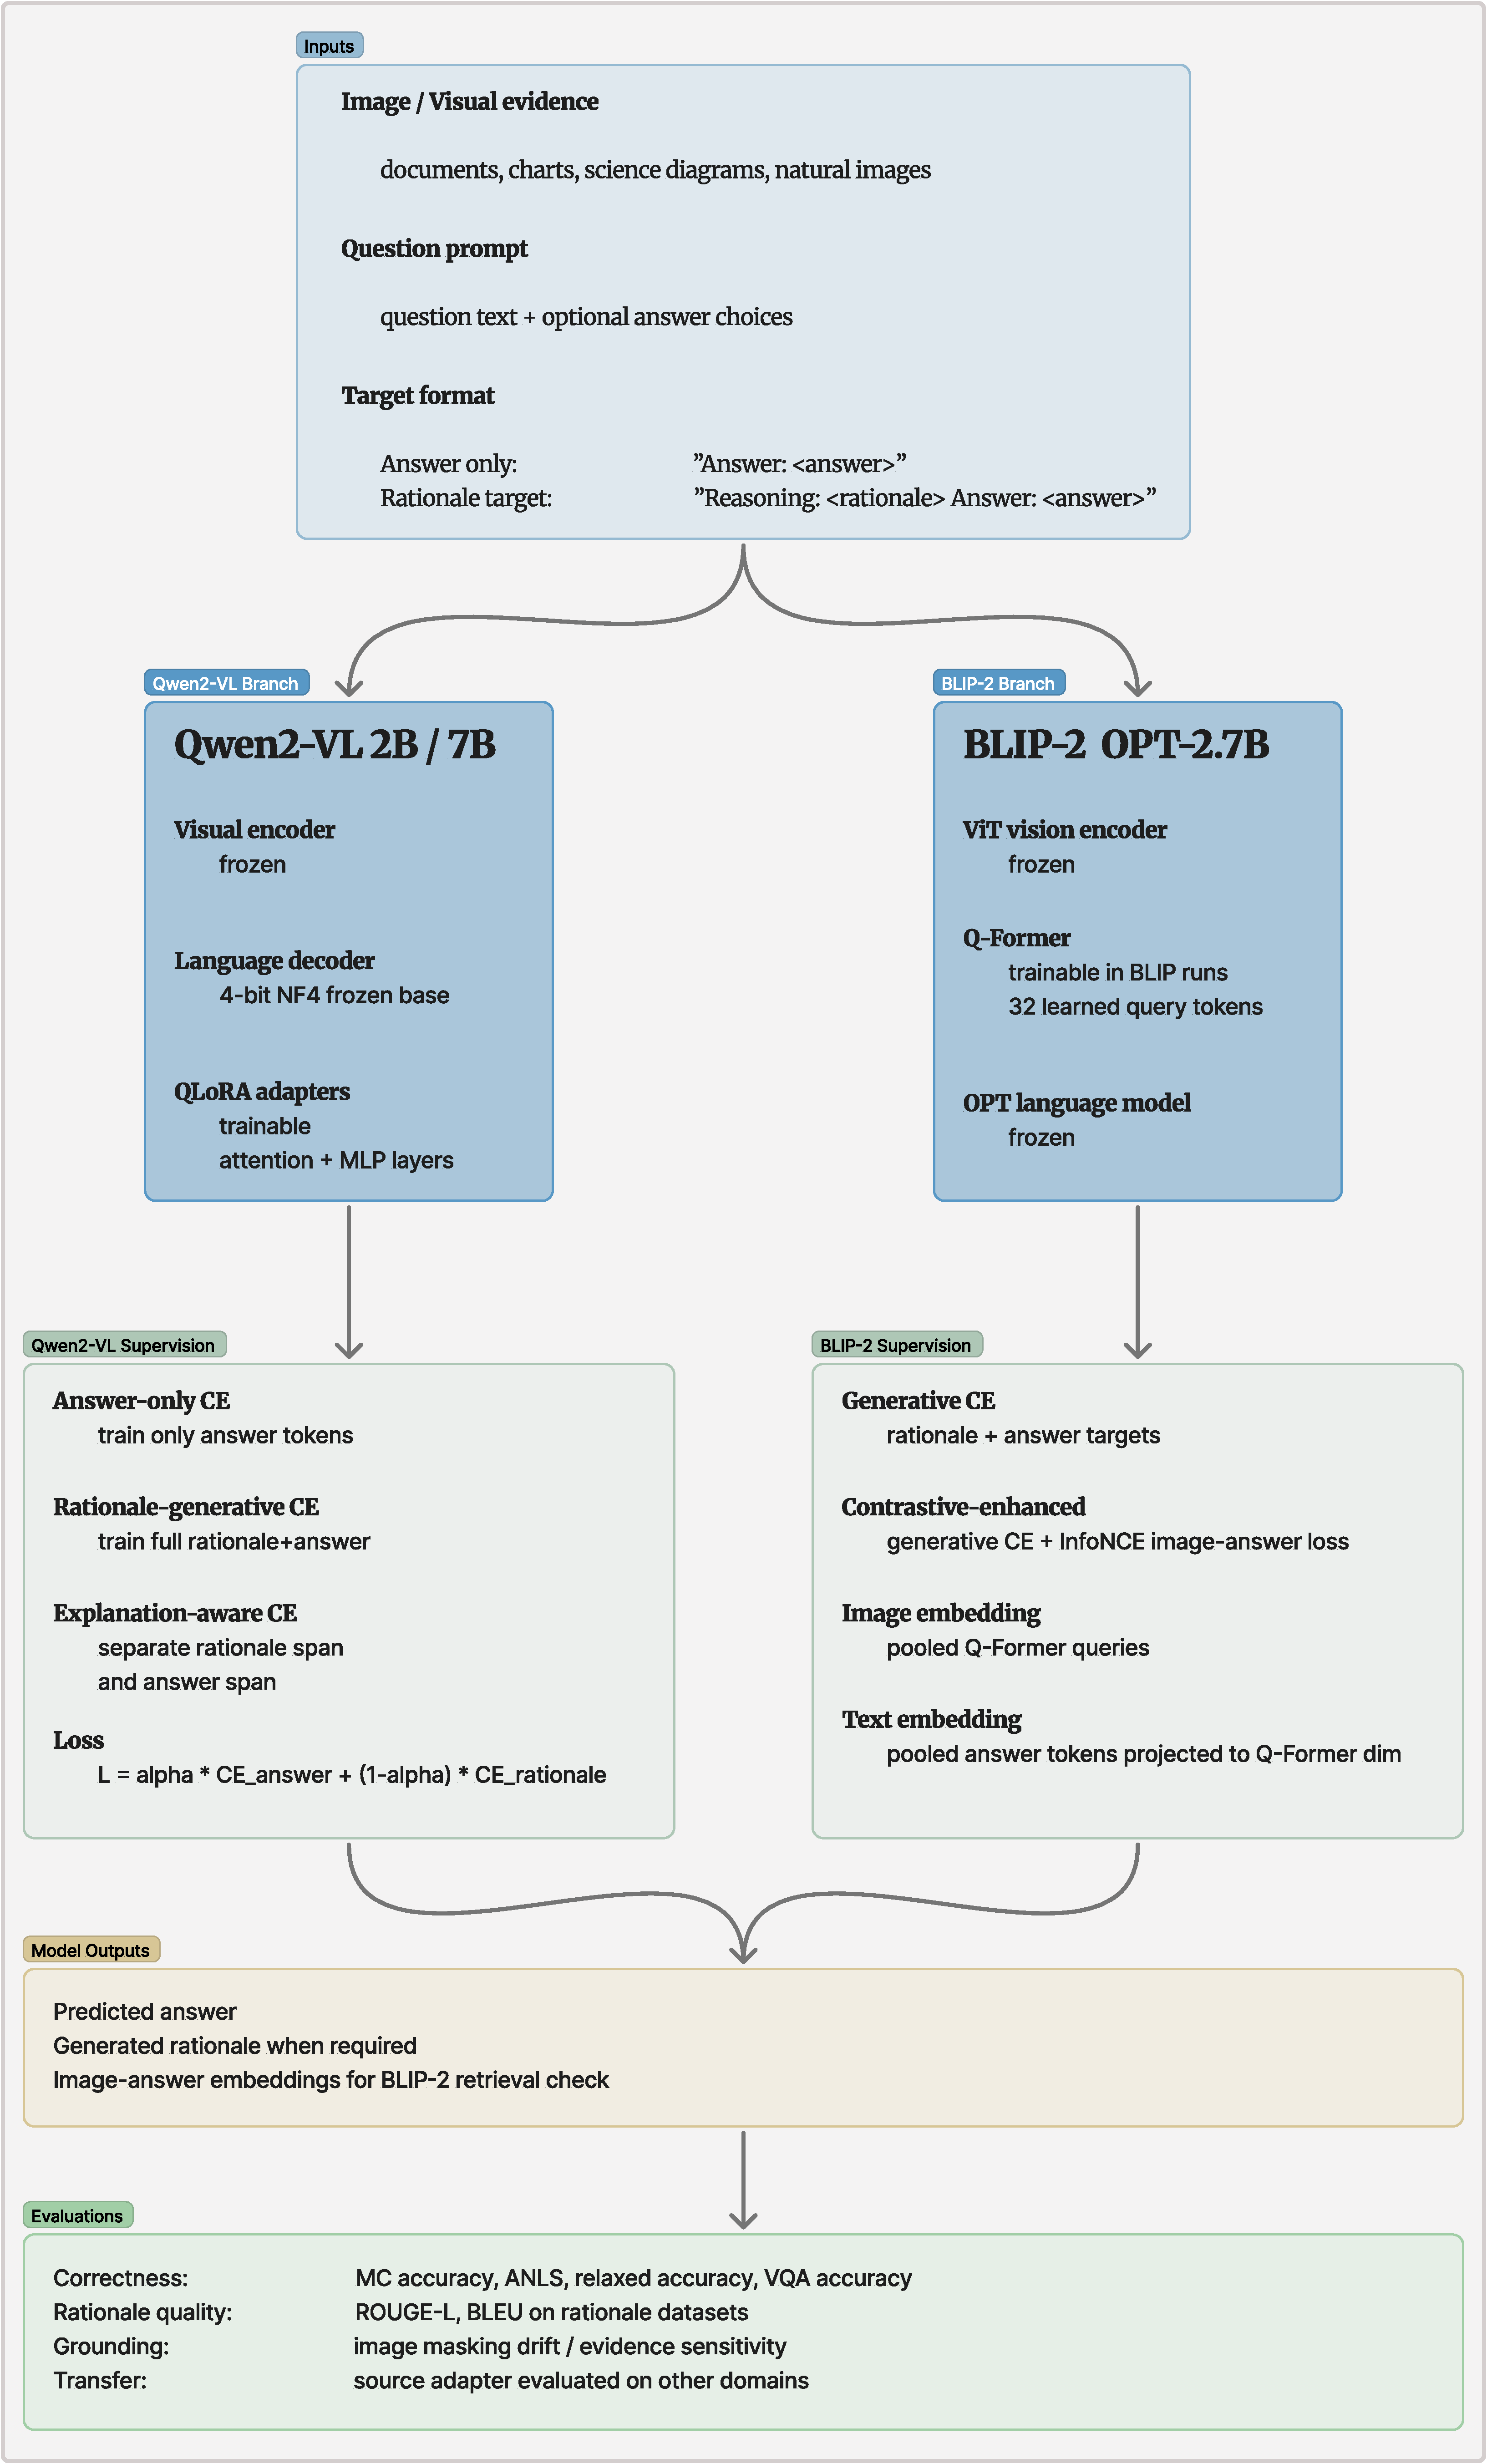
\includegraphics[height=0.74\textheight,keepaspectratio]{./Figures/icons/Architecture_cropped}}
\caption{Model-level architecture for explanation-aware cross-modal alignment.
Visual evidence and the question prompt are encoded into a multimodal token stream.
The Qwen2-VL path uses trainable QLoRA adapters and separate rationale and answer supervision spans.
The BLIP-2 path keeps the vision tower and OPT language model frozen and trains the Q-Former-side generative or contrastive alignment components.}
\label{Fig:Architecture}
\end{figure*}

\begin{equation}
    \mathcal{L} = \alpha\,\mathcal{L}_{\text{answer}} + (1-\alpha)\,\mathcal{L}_{\text{explanation}}
    \label{Eq:Loss}
\end{equation}
where $\mathcal{L}_{\text{answer}}$ and $\mathcal{L}_{\text{explanation}}$ are the masked cross-entropy losses over the answer and explanation token spans, and $\alpha$ controls their relative weight.
There are two alpha modes.
Fixed-alpha mode treats $\alpha$ as a dial we set by configuration, an ablation knob.
Length-aware mode does something different: it derives the effective answer weight straight from the supervised token counts:

\begin{equation}
    \alpha_{\text{eff}} =
    \frac{\lambda\,n_{\text{answer}}}{\lambda\,n_{\text{answer}} + n_{\text{explanation}}},
    \label{Eq:LengthAlpha}
\end{equation}
where $n_{\text{answer}}$ and $n_{\text{explanation}}$ are the answer and explanation token counts after collation, and $\lambda$ is the answer-weight multiplier.
With $\lambda=1$, this collapses to plain uniform token-level cross-entropy over the rationale-plus-answer target.
So the fixed-alpha sweep is the ablation; the length-aware run is the audit control for the natural, token-weighted setting.

Multiple-choice datasets are scored in two steps at inference.
First the model writes a short reasoning trace from the image and question.
Then, in the context of that trace, each candidate answer gets a length-normalised conditional likelihood, and the highest score wins.
The two-step design is there to avoid brittle string parsing and option-label copying.
Open-ended datasets are simpler: the generated answer string is scored with the dataset's native metric.
Whenever the model produces a rationale, we save it, and those saved rationales feed the text-quality and faithfulness analysis.

\subsection{Evaluation metrics}
Evaluation splits into three parts: answer quality, rationale quality, and evidence sensitivity.
Answer quality always uses the benchmark's own native metric.
When the tables say ``headline metric,'' they mean exactly that native primary metric for the target dataset, not some universal number to be read straight across datasets.
For ScienceQA and A-OKVQA that metric is multiple-choice accuracy.
DocVQA uses average normalised Levenshtein similarity (ANLS), per the benchmark convention~\cite{mathew2021docvqa}.
ChartQA uses relaxed accuracy on numerical answers~\cite{masry2022chartqa}.
The VQAv2 subset uses VQA consensus accuracy wherever annotator answers exist~\cite{antol2015vqa,goyal2017vqav2}.
Rationale quality leans on BLEU and ROUGE-L whenever gold rationales are available~\cite{papineni2002bleu,lin2004rouge}.
Neither is a perfect judge, but together they give a basic lexical and sequence-level check on the explanation.
Evidence sensitivity asks a blunter question: does the answer's likelihood move when we mask part of the image? This borrows the old idea of occlusion sensitivity analysis~\cite{zeiler2014visualizing}.
The specific measure is evidence-masking consistency, written out in Equation~\ref{Eq:Drift}.
The qualitative diagnostic then lines up the high-drift regions against whatever visual evidence the generated explanation actually names, when that comparison is possible.

\begin{equation}
    \mathrm{drift}(r) = s\!\left(a \mid I\right) - s\!\left(a \mid I \setminus r\right)
    \label{Eq:Drift}
\end{equation}
where $s(a \mid I)$ is the length-normalised log-likelihood of the gold answer $a$ given image $I$, and $I \setminus r$ is the same image with region $r$ occluded.
A large positive drift says the masked region mattered.
A drift near zero says the opposite: the answer probably leaned on language priors, a shortcut, or non-visual context.
The absolute scale does not travel across datasets, since answer length, prompt family, image resolution, and task format all bend the likelihood scores.
The split it captures is the familiar one between a useful explanation and a faithful one.
It also speaks to recent hallucination and critique work, where a model happily describes or relies on visual content that simply is not there~\cite{guan2024hallusionbench,jiang2024hacl,wu2025visco,zhang2025criticv}.
That is why evidence sensitivity sits next to answer accuracy here, rather than being parked as a post-hoc example.

\subsection{Experimental settings}
Every variant runs under the same fixed-budget protocol, and any deviation from it is written into the experiment ledger.
The Qwen2-VL runs share one recipe: AdamW, a learning rate of $2 \times 10^{-4}$, cosine decay, three percent warm-up, weight decay of 0.01, bf16 compute, and an effective batch size of 32 reached through gradient accumulation.
The base model loads under 4-bit NormalFloat (NF4) quantisation.
Unless a result table says otherwise, the QLoRA adapters use rank 16 and scaling factor 32~\cite{hu2022lora,dettmers2023qlora}.
The workhorse backbone is Qwen2-VL-2B-Instruct, strong enough for the target tasks yet small enough to fit the budget~\cite{wang2024qwen2vl}.
For BLIP-2 we use Salesforce BLIP-2 OPT-2.7B, vision tower and OPT language model frozen, training only the Q-Former-side alignment components~\cite{li2023blip2}.
The scale ablation reuses the same QLoRA recipe on Qwen2-VL-7B.
Each run logs its dataset split, filtered count, seed, objective, adapter configuration, and metrics.
The pipeline also writes a split-and-leakage audit from the selected train and evaluation identifiers, wherever the dataset exposes stable IDs.
For the capped datasets in the final artifact set, that overlap count comes back at zero.
DocVQA is the one non-standard split: the loaded dataset only exposes validation and test, so the controlled run trains on \texttt{validation[:80\%]} and evaluates on \texttt{validation[80\%:]}, with native-ID overlap checking.
The audit shows zero native-ID overlap, but it cannot prove document-level disjointness past the IDs the loader exposes.
So we treat the DocVQA number as a capped internal adaptation result, not a public-test benchmark claim.
We also attach approximate uncertainty estimates to the accuracy-style headline metrics.
With most evaluation caps at 200 examples and only a few seeds in the budget, a gap like 0.790 versus 0.795 is an observed difference, nothing more.
Table~\ref{tab:Config} lists the default configuration.

\begin{table}[!ht]
\centering
\caption{Default Qwen2-VL QLoRA fine-tuning configuration. BLIP-2 contrastive runs use the separately reported frozen-vision/frozen-LLM Q-Former training setup. Any run that changes these values is reported separately in the experiment ledger and in the Results section.}
\label{tab:Config}
\begin{tabular}{|l|c|}
\hline
\multicolumn{2}{|c|}{\textbf{Training Configuration}} \\ \hline
Adapter & QLoRA (4-bit NF4, rank 16, scaling 32) \\
Optimizer & AdamW ($\beta_1$=0.9, $\beta_2$=0.999) \\
Learning rate & $2 \times 10^{-4}$ (cosine, 3\% warm-up) \\
Weight decay & 0.01 \\
Effective batch size & 32 with gradient accumulation \\
Precision & bf16 compute \\
Primary seed policy & one seed per complete configuration \\ \hline
\end{tabular}
\end{table}

\subsection{Experiment ledger}
Before any scores, Table~\ref{tab:ExperimentLedger} lays out the comparisons.
The line that matters is rationale availability.
ScienceQA and A-OKVQA can carry rationale-generative and explanation-aware supervision, because they ship gold rationales.
ChartQA, DocVQA, and VQAv2 stay on answer-only fallback, plus the transfer and domain runs, until some future experiment adds rationale supervision of their own.

\begin{table*}[!ht]
\centering
\caption{Main experiment ledger. The full generated ledger includes exact caps, seeds, prompt variants, alpha mode, and configuration hashes.}
\label{tab:ExperimentLedger}
\small
\renewcommand{\arraystretch}{1.15}
\begin{tabular}{|>{\raggedright\arraybackslash}p{0.20\textwidth}|>{\raggedright\arraybackslash}p{0.36\textwidth}|>{\raggedright\arraybackslash}p{0.34\textwidth}|}
\hline
\textbf{Comparison} & \textbf{Runs included} & \textbf{Use in the paper} \\ \hline
BLIP-2 objective pair & BLIP-2 OPT-2.7B on ScienceQA: generative and generative+contrastive. & Tests whether the auxiliary contrastive objective adds anything beyond BLIP-2 generative fine-tuning. \\
ScienceQA controls & Qwen2-VL-2B on ScienceQA: answer-only, rationale+answer CE, fixed-$\alpha$ explanation-aware sweep, and length-aware control. & Separates answer supervision, rationale supervision, and alpha weighting on a gold-rationale dataset. \\
A-OKVQA controls & Qwen2-VL-2B on A-OKVQA: answer-only, rationale+answer CE, fixed-$\alpha$ explanation-aware, and length-aware control. & Repeats the rationale-supervision comparison on a second gold-rationale domain. \\
Fallback domains & Qwen2-VL-2B on ChartQA, DocVQA, and VQAv2 with answer-only fallback prompts. & Reports in-domain adaptation and transfer for datasets without gold rationales; these rows are not used as explanation-aware evidence. \\
Scale & Qwen2-VL-2B and Qwen2-VL-7B on ScienceQA with the same fixed explanation-aware QLoRA setting. & Checks whether the selected setup changes when the backbone scale increases. \\
Transfer & Qwen2-VL-2B source adapters evaluated on target-domain prompts across all datasets. & Tests cross-domain behaviour separately from the official in-domain result table. \\
Masking & Selected Qwen2-VL runs with image-region perturbation and saved visual examples. & Measures evidence sensitivity beside answer accuracy and rationale quality. \\ \hline
\end{tabular}
\end{table*}

\FloatBarrier

\section{Results}
The results track the comparison types from the ledger, in order.
The BLIP-2 objective pair comes first, testing whether the auxiliary contrastive term earns its place beyond generative fine-tuning.
Then the ScienceQA and A-OKVQA runs pull answer-only, rationale-generative, and explanation-aware supervision apart on the two datasets that have gold rationales.
The chart, document, and VQAv2 runs follow, showing in-domain adaptation where no gold rationales exist.
After that come masking-based evidence sensitivity, the Qwen2-VL scale check, and cross-domain transfer.
One reminder throughout: every score comes from the capped single-seed protocol above, so they are controlled framework results, not leaderboard numbers.

\subsection{Objective-level comparison}
Table~\ref{tab:objective_comparison} holds the direct objective comparisons.
Take the BLIP-2 ScienceQA pair first: both trained variants clear the 0.445 frozen baseline, the contrastive-enhanced run landing at 0.480 and the generative control at 0.475.
That gap is tiny, and it sits inside the approximate uncertainty intervals in Table~\ref{tab:uncertainty}.
Retrieval tells the same cautious story: the contrastive-enhanced model posts recall@1 (R@1) of 0.010, R@5 of 0.020, R@10 of 0.030, and a mean reciprocal rank (MRR) of 0.0307.
Qwen2-VL-2B is stronger across the board.
Rationale-generative fine-tuning reaches 0.780 on ScienceQA and 0.790 on A-OKVQA.
On A-OKVQA the explanation-aware run reaches 0.795 accuracy, 0.337 ROUGE-L, and 0.087 BLEU, numerically a hair above the generative control, which we read as an observed single-run difference rather than a settled win.
The honest surprise is the answer-only controls: 0.800 on ScienceQA and 0.830 on A-OKVQA, both strong.
The zero-shot column, meanwhile, is one shared backbone--dataset reference for orientation, not a fresh prompt-family baseline per row.
Back on ScienceQA, the fixed $\alpha=0.50$ explanation-aware run reaches 0.765.
The length-aware control reaches 0.780, level with the rationale-generative control but still under the answer-only number.

\begin{table*}[!ht]
\centering
\caption{Objective-level results under the controlled protocol. The zero-shot reference is the shared pre-fine-tuning score for the same backbone and dataset group, not a separately recomputed frozen score for every prompt family. Accuracy is multiple-choice accuracy for ScienceQA and A-OKVQA.}
\label{tab:objective_comparison}
\scriptsize
\begin{adjustbox}{max width=\textwidth}
\begin{tabular}{|l|l|l|c|c|c|c|}
\hline
\textbf{Backbone} & \textbf{Dataset} & \textbf{Objective} & \textbf{Zero-shot ref.} & \textbf{Final} & \textbf{ROUGE-L} & \textbf{BLEU} \\ \hline
BLIP-2 OPT-2.7B & ScienceQA & Generative & 0.445 & 0.475 & -- & -- \\
BLIP-2 OPT-2.7B & ScienceQA & Contrastive-enhanced & 0.445 & 0.480 & -- & -- \\
Qwen2-VL-2B & ScienceQA & Answer-only & 0.400 & \textbf{0.800} & -- & -- \\
Qwen2-VL-2B & ScienceQA & Rationale+answer CE & 0.400 & 0.780 & 0.693 & 0.559 \\
Qwen2-VL-2B & ScienceQA & Explanation-aware, $\alpha=0.50$ & 0.400 & 0.765 & 0.643 & 0.493 \\
Qwen2-VL-2B & ScienceQA & Explanation-aware, length-aware & 0.400 & 0.780 & 0.696 & 0.563 \\
Qwen2-VL-2B & A-OKVQA & Answer-only & 0.355 & \textbf{0.830} & -- & -- \\
Qwen2-VL-2B & A-OKVQA & Rationale+answer CE & 0.355 & 0.790 & 0.329 & 0.083 \\
Qwen2-VL-2B & A-OKVQA & Explanation-aware, $\alpha=0.50$ & 0.355 & 0.795 & 0.337 & 0.087 \\
Qwen2-VL-2B & A-OKVQA & Explanation-aware, length-aware & 0.355 & 0.790 & 0.330 & 0.083 \\ \hline
\end{tabular}
\end{adjustbox}
\end{table*}

\begin{table*}[!ht]
\centering
\caption{Approximate uncertainty for selected accuracy-style headline metrics. These intervals use the generated normal-approximation standard errors for capped evaluation sets, so they are a caution about small observed differences rather than a replacement for multi-seed testing.}
\label{tab:uncertainty}
\scriptsize
\begin{adjustbox}{max width=\textwidth}
\begin{tabular}{|l|l|c|c|c|}
\hline
\textbf{Run} & \textbf{Metric} & \textbf{Eval cap} & \textbf{Score} & \textbf{Approx. 95\% CI} \\ \hline
BLIP-2 generative ScienceQA & MC accuracy & 200 & 0.475 & 0.406--0.544 \\
BLIP-2 contrastive ScienceQA & MC accuracy & 200 & 0.480 & 0.411--0.549 \\
ScienceQA answer-only & MC accuracy & 200 & 0.800 & 0.745--0.855 \\
ScienceQA rationale+answer CE & MC accuracy & 200 & 0.780 & 0.723--0.837 \\
ScienceQA explanation-aware, $\alpha=0.50$ & MC accuracy & 200 & 0.765 & 0.706--0.824 \\
ScienceQA explanation-aware, length-aware & MC accuracy & 200 & 0.780 & 0.723--0.837 \\
A-OKVQA answer-only & MC accuracy & 200 & 0.830 & 0.778--0.882 \\
A-OKVQA rationale+answer CE & MC accuracy & 200 & 0.790 & 0.734--0.847 \\
A-OKVQA explanation-aware, $\alpha=0.50$ & MC accuracy & 200 & 0.795 & 0.739--0.851 \\
Qwen2-VL-7B ScienceQA, $\alpha=0.50$ & MC accuracy & 200 & 0.885 & 0.841--0.929 \\ \hline
\end{tabular}
\end{adjustbox}
\end{table*}

\begin{figure}[!ht]
\centerline{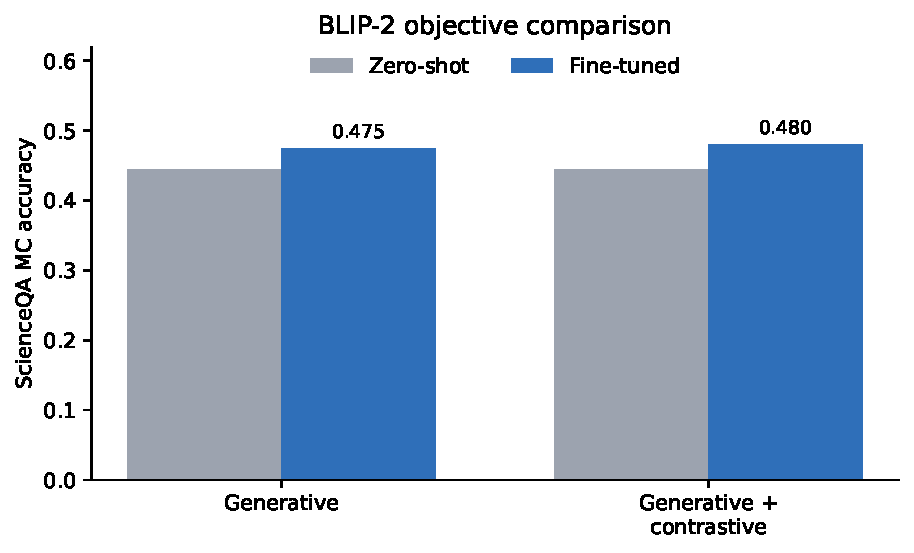
\includegraphics[width=0.82\linewidth]{./Figures/generated/blip2_objective}}
\caption{BLIP-2 generative and contrastive-enhanced ScienceQA results.
Both runs improve over the frozen baseline, with only a small observed gain from the auxiliary contrastive term.}
\label{Fig:BlipObjective}
\end{figure}

\begin{figure}[!ht]
\centerline{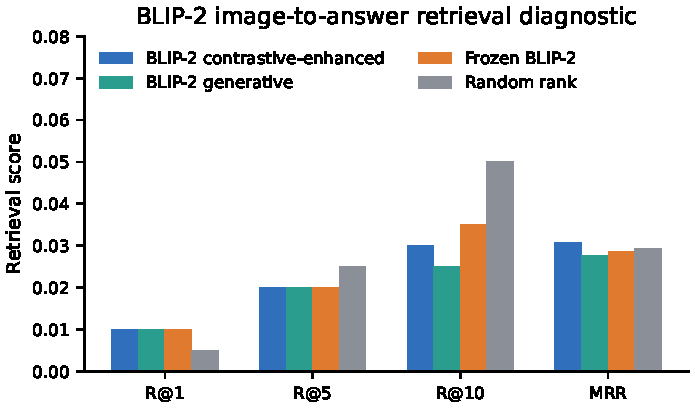
\includegraphics[width=0.82\linewidth]{./Figures/generated/contrastive_retrieval}}
\caption{BLIP-2 image-to-answer retrieval diagnostic.
The analysis reports frozen BLIP-2, BLIP-2 generative, BLIP-2 contrastive-enhanced, and random-rank controls so the contrastive branch is not interpreted without a reference point.}
\label{Fig:ContrastiveRetrieval}
\end{figure}

\begin{figure}[!ht]
\centerline{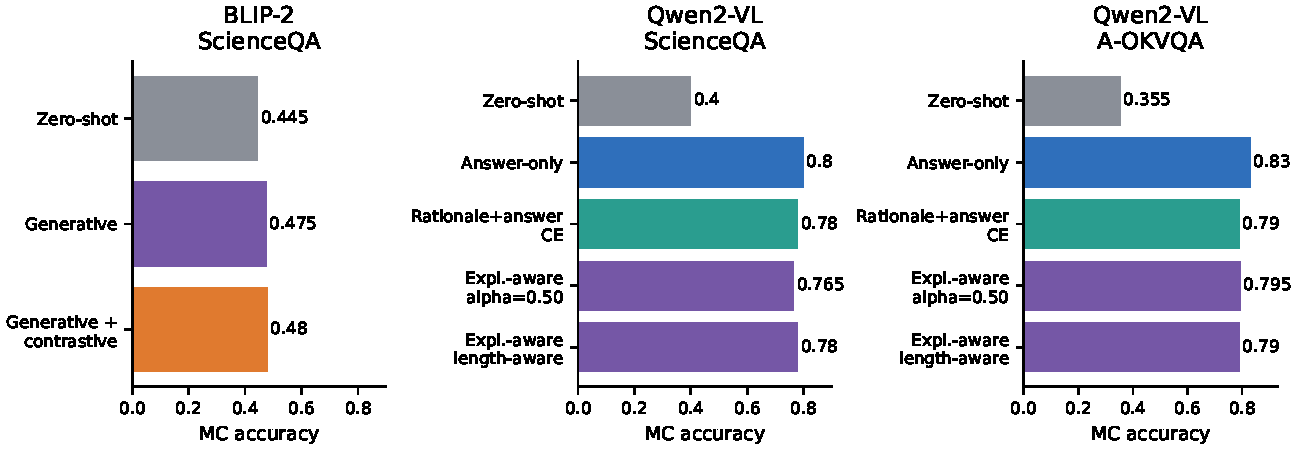
\includegraphics[width=\linewidth]{./Figures/generated/controlled_strategy_comparison}}
\caption{Controlled strategy comparison for BLIP-2 and Qwen2-VL.
The figure shows zero-shot, answer-only, rationale-generative, explanation-aware, and contrastive variants where those controls are available.}
\label{Fig:ObjectiveComparison}
\end{figure}

\FloatBarrier

\subsection{Effect of explanation-aware training}
Table~\ref{tab:alpha_sweep} and Figure~\ref{Fig:AlphaSweep} trace the ScienceQA $\alpha$-sweep, where $\alpha$ is the answer-span weight from Equation~\ref{Eq:Loss}.
Fine-tuning alone lifts accuracy from the 0.400 zero-shot reference into the 0.690--0.780 band.
The sweet spot is low: $\alpha=0.10$, at 0.780.
Push $\alpha$ toward the answer-heavy end and accuracy slides, to 0.690 at $\alpha=0.75$ and 0.695 at $\alpha=1.00$.
The explanation metrics move in lockstep.
ROUGE-L and BLEU also peak at $\alpha=0.10$ (0.695 and 0.566) and decay as $\alpha$ climbs.
At $\alpha=1.00$ only the answer span is supervised inside a rationale-shaped target, so there are no rationale metrics to report.
In accuracy, the $\alpha=0.10$ run ties the rationale-generative and length-aware controls.
One trap worth flagging: the $\alpha=1.00$ row is not the true answer-only control, because the model still sees a rationale-shaped template even though the rationale span goes unsupervised.
The genuine answer-only ScienceQA control, on its own prompt family, reaches 0.800.
And all of this rests on one seed, 2{,}000 training and 200 evaluation examples, so these are observed effects, not final statistical proof.

\begin{table}[!ht]
\centering
\caption{Explanation-aware fixed-$\alpha$ sweep on ScienceQA (Qwen2-VL-2B, QLoRA, 2{,}000 train / 200 eval, single seed). The coefficient $\alpha$ weights the answer span in Equation~\ref{Eq:Loss}: $\alpha=1$ is answer-span-only within the rationale target and $\alpha=0$ is explanation-span-only. The zero-shot and rationale-generative rows are references. Random-choice accuracy is 0.354. The best fixed $\alpha$ is shown in bold.}
\label{tab:alpha_sweep}
\begin{tabular}{|l|c|c|c|}
\hline
\textbf{Variant ($\alpha$)} & \textbf{MC accuracy} & \textbf{ROUGE-L} & \textbf{BLEU} \\ \hline
Zero-shot (frozen) & 0.400 & -- & -- \\
Rationale+answer CE & \textbf{0.780} & 0.693 & 0.559 \\ \hline
$\alpha=0.00$ (explanation-only) & 0.725 & 0.417 & 0.299 \\
$\alpha=0.10$ & \textbf{0.780} & \textbf{0.695} & \textbf{0.566} \\
$\alpha=0.25$ & 0.775 & 0.686 & 0.548 \\
$\alpha=0.50$ & 0.765 & 0.643 & 0.493 \\
$\alpha=0.75$ & 0.690 & 0.604 & 0.443 \\
$\alpha=1.00$ (answer-span only) & 0.695 & -- & -- \\ \hline
\end{tabular}
\end{table}

\begin{figure}[!ht]
\centerline{
\includegraphics[width=0.82\linewidth]{./Figures/generated/alpha_sweep}}
\caption{Fixed-alpha explanation-aware sweep on ScienceQA.
Answer accuracy peaks at the low-answer-weight setting and declines toward both extremes inside the rationale-plus-answer target.
Explanation quality (ROUGE-L, BLEU) peaks at the same point and falls as $\alpha$ increases.
Series are distinguished by marker shape and line style; the dashed grey line marks random-choice accuracy. Single seed.}
\label{Fig:AlphaSweep}
\end{figure}

\FloatBarrier

\subsection{Domain-level behaviour}
Table~\ref{tab:domain_results} and Figure~\ref{Fig:CrossDomain} gather the selected domain runs from the final matrix.
For ScienceQA the row uses the fixed $\alpha=0.50$ explanation-aware run, so it lines up with the in-domain figure; the stronger $\alpha=0.10$ and length-aware settings live in the sweep table above.
The biggest jumps land on DocVQA, VQAv2, ChartQA, and A-OKVQA.
A-OKVQA climbs from 0.355 to 0.795 accuracy against the reported zero-shot reference.
The VQAv2 subset goes from 0.350 to 0.730 VQA accuracy.
ChartQA reaches 0.655 relaxed accuracy, exact match 0.410.
DocVQA is the headline, at 0.905 ANLS with exact match at 0.855.
That number is strong for a capped internal run, but it deserves caution on three counts: the qualitative samples are short extractive answers, the setup is answer-only fallback rather than gold rationales, and the split audit cannot prove document-level disjointness past the native IDs it can see.

\begin{table*}[!ht]
\centering
\caption{Domain-level results for the completed Qwen2-VL-2B runs. Each domain uses its native headline metric: multiple-choice accuracy for ScienceQA and A-OKVQA, relaxed accuracy for ChartQA, ANLS for DocVQA, and VQA accuracy for the VQAv2 subset.}
\label{tab:domain_results}
\scriptsize
\begin{adjustbox}{max width=\textwidth}
\begin{tabular}{|l|l|l|c|c|c|}
\hline
\textbf{Domain} & \textbf{Dataset} & \textbf{Objective} & \textbf{Zero-shot ref.} & \textbf{Final} & \textbf{Secondary metric} \\ \hline
Science & ScienceQA & Explanation-aware, $\alpha=0.50$ & 0.400 & 0.765 & ROUGE-L 0.643, BLEU 0.493 \\
Commonsense & A-OKVQA & Explanation-aware, $\alpha=0.50$ & 0.355 & 0.795 & ROUGE-L 0.337, BLEU 0.087 \\
Charts & ChartQA & Answer-only fallback & 0.335 & 0.655 & Exact match 0.410 \\
Documents & DocVQA & Answer-only fallback & 0.349 & 0.905 & Exact match 0.855 \\
Natural images & VQAv2 subset & Answer-only fallback & 0.350 & 0.730 & Exact match 0.350 $\rightarrow$ 0.730 \\ \hline
\end{tabular}
\end{adjustbox}
\end{table*}

\begin{figure}[!ht]
\centerline{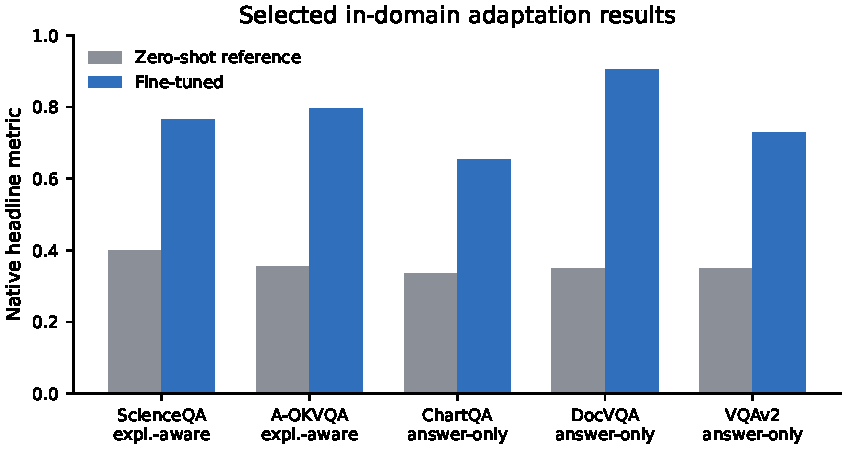
\includegraphics[width=0.82\linewidth]{./Figures/generated/cross_domain}}
\caption{In-domain adaptation results for the selected completed Qwen2-VL-2B domain runs.
The comparison mixes rationale-supervised ScienceQA/A-OKVQA rows with answer-only fallback rows for domains without gold rationales, so it should not be read as an explanation-aware effect across all domains.}
\label{Fig:CrossDomain}
\end{figure}

\FloatBarrier

\subsection{Faithfulness and hallucination analysis}
Table~\ref{tab:faithfulness} and Figure~\ref{Fig:Faithfulness} carry the evidence-masking drift check.
Each number is a mean over 30 evaluation examples.
The bigger and more positive it is, the more masking a region costs the gold-answer likelihood, which means the model was relying on what we hid.
The drift piles up on the structured tasks: DocVQA at 0.375, ChartQA at 0.224, VQAv2 at 0.111.
ScienceQA and A-OKVQA usually sit far lower, with one loud exception, the ScienceQA answer-only adapter at 0.0898.
That low ScienceQA drift is not surprising; the questions come loaded with language priors and explicit answer choices, the visual evidence is diffuse, and a coarse mask can miss the single cue the model actually used.
Explanation supervision does not move drift in any clean way here.
At $\alpha=0.10$ it is 0.0223, at $\alpha=0.50$ it is 0.0197, and answer-span-only $\alpha=1.00$ gives 0.0149, despite that run producing no supervised rationale at all.
On A-OKVQA the explanation-aware run drifts a touch more than the generative control, 0.0271 against 0.0245, but the intervals around both are wide.
Read plainly, the masking result backs a domain-sensitivity story, not the sweeping claim that explanation-aware training by itself buys faithfulness.
We report no manual hallucination rate, because we never ran a fixed annotation protocol for hallucination categories.

\begin{table}[!ht]
\centering
\caption{Evidence-masking drift by completed run. Higher values indicate stronger sensitivity to masked visual evidence. The intervals are approximate 95\% intervals from the generated masking artifact.}
\label{tab:faithfulness}
\scriptsize
\begin{adjustbox}{max width=\textwidth}
\begin{tabular}{|l|c|c|c|}
\hline
\textbf{Run} & \textbf{Mean drift} & \textbf{Approx. 95\% CI} & \textbf{Examples} \\ \hline
ScienceQA answer-only & 0.0898 & 0.0197--0.1830 & 30 \\
ScienceQA rationale+answer CE & 0.0217 & -0.0100--0.0582 & 30 \\
ScienceQA $\alpha=0.10$ & 0.0223 & -0.0080--0.0568 & 30 \\
ScienceQA $\alpha=0.50$ & 0.0197 & -0.0119--0.0552 & 30 \\
ScienceQA answer-span-only $\alpha=1.00$ & 0.0149 & -0.0274--0.0638 & 30 \\
A-OKVQA rationale+answer CE & 0.0245 & -0.0236--0.0726 & 30 \\
A-OKVQA explanation-aware & 0.0271 & -0.0075--0.0627 & 30 \\
ChartQA answer-only fallback & 0.2237 & 0.1419--0.3140 & 30 \\
DocVQA answer-only fallback & 0.3749 & 0.2770--0.4960 & 30 \\
VQAv2 answer-only fallback & 0.1109 & 0.0274--0.2408 & 30 \\
Qwen2-VL-7B ScienceQA $\alpha=0.50$ & 0.0114 & -0.0059--0.0260 & 30 \\ \hline
\end{tabular}
\end{adjustbox}
\end{table}

\begin{figure}[!ht]
\centerline{
\includegraphics[width=0.82\linewidth]{./Figures/generated/faithfulness}}
\caption{Mean evidence-masking drift across completed runs.
Structured document and chart runs show much stronger visual sensitivity than the rationale-rich ScienceQA and A-OKVQA runs, but stronger drift does not automatically imply better answer accuracy.}
\label{Fig:Faithfulness}
\end{figure}

\IfFileExists{./Figures/generated/masking_example_chartqa_clean.pdf}{
\begin{figure*}[!ht]
\centerline{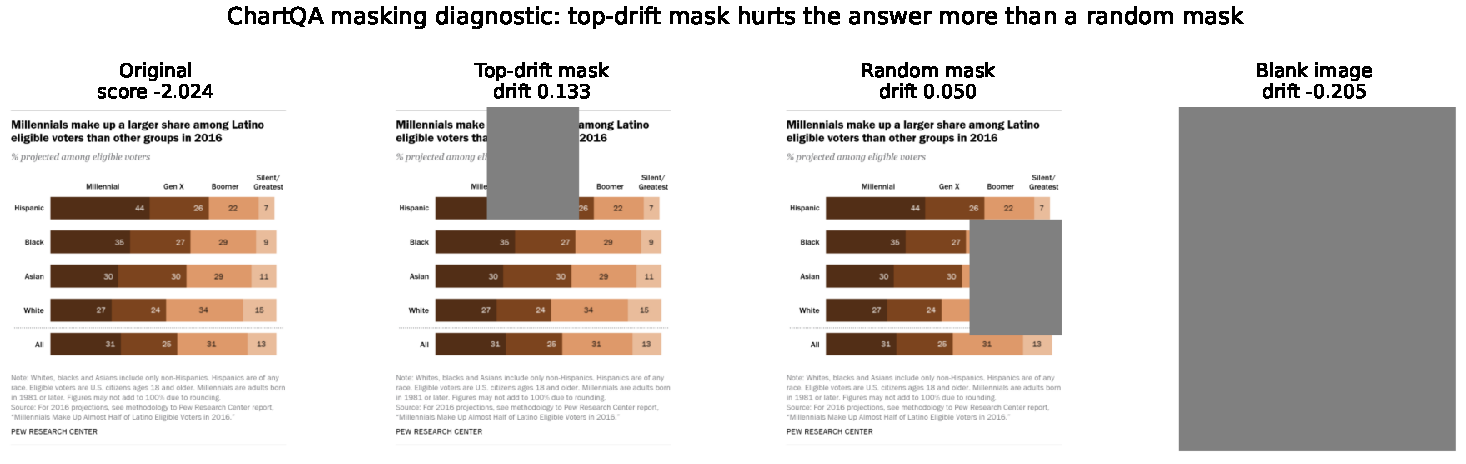
\includegraphics[width=\linewidth]{./Figures/generated/masking_example_chartqa_clean}}
\caption{Example masking diagnostic for a ChartQA answer-only fallback run.
The pipeline saves the original image, the top-drift mask, a random-region mask, and a blank-image control, together with the full-image and masked answer scores.
This figure is used as an evidence-sensitivity example, not as proof that a generated rationale is faithful.}
\label{Fig:MaskingExample}
\end{figure*}
}{}

\FloatBarrier

\subsection{Efficiency and scale trade-offs}
Table~\ref{tab:scale} and Figure~\ref{Fig:Scale} put Qwen2-VL-2B and Qwen2-VL-7B side by side on the same ScienceQA explanation-aware setting ($\alpha=0.50$).
Scaling up pays.
The 7B run lifts accuracy from 0.765 to 0.885.
ROUGE-L rises from 0.643 to 0.738, BLEU from 0.493 to 0.637.
It is the single largest gain anywhere in the completed set.
Both runs still fit under QLoRA.
What the logs do not give us is a stable wall-clock or peak-memory figure, so this stands as a model-scale result, not a precise efficiency one.

\begin{table}[!ht]
\centering
\caption{Qwen2-VL scale comparison on ScienceQA with the same explanation-aware objective ($\alpha=0.50$).}
\label{tab:scale}
\begin{tabular}{|l|c|c|c|}
\hline
\textbf{Model} & \textbf{MC accuracy} & \textbf{ROUGE-L} & \textbf{BLEU} \\ \hline
Qwen2-VL-2B & 0.765 & 0.643 & 0.493 \\
Qwen2-VL-7B & \textbf{0.885} & \textbf{0.738} & \textbf{0.637} \\ \hline
\end{tabular}
\end{table}

\begin{figure}[!ht]
\centerline{
\includegraphics[width=0.82\linewidth]{./Figures/generated/scale_comparison}}
\caption{Scale comparison for the fixed ScienceQA explanation-aware setting.
Moving from Qwen2-VL-2B to Qwen2-VL-7B improves both answer accuracy and rationale-overlap metrics.}
\label{Fig:Scale}
\end{figure}

\FloatBarrier

\subsection{Cross-domain transfer}
Table~\ref{tab:transfer} and Figure~\ref{Fig:Transfer} lay out the train-domain against test-domain transfer matrix.
Every column is scored in its target domain's own metric, so the only safe comparisons run down a column, not across a row.
Where the controls exist, the matrix keeps answer-only, rationale-generative, and explanation-aware sources separate.
Treat it as an evaluation probe rather than the official in-domain table; a diagonal cell can drift a little from the matching completed run when the transfer evaluator routes through a different prompt family.
The probe matters because answer-only training often travels better than rationale-generative training.
The ScienceQA answer-only adapter is the clearest case, reaching 0.805 on A-OKVQA, 0.645 on ChartQA, 0.703 on DocVQA, and 0.630 on VQAv2.
Its rationale-generative and explanation-aware siblings clear the random baselines but fall off on ChartQA, DocVQA, and VQAv2.
A-OKVQA sources split the honours: rationale-generative training wins DocVQA transfer in that group at 0.764, while answer-only wins VQAv2 at 0.700.
DocVQA is strongest at home (0.910), and the document-trained adapter carries over to ChartQA too (0.685).
The pattern, in short: transfer depends on the target domain and the source objective together, not on domain alone.

\begin{table*}[!ht]
\centering
\caption{Cross-domain transfer matrix. Rows indicate the training domain and columns indicate the evaluation domain. Each column uses the target domain's headline metric, so values are best compared within a column.}
\label{tab:transfer}
\scriptsize
\begin{adjustbox}{max width=\textwidth}
\begin{tabular}{|l|ccccc|}
\hline
\textbf{Trained on} & \textbf{ScienceQA} & \textbf{A-OKVQA} & \textbf{ChartQA} & \textbf{DocVQA} & \textbf{VQAv2} \\ \hline
ScienceQA answer-only & 0.800 & 0.805 & 0.645 & 0.703 & 0.630 \\
ScienceQA rationale CE & 0.780 & 0.760 & 0.450 & 0.559 & 0.300 \\
ScienceQA explanation-aware & 0.740 & 0.765 & 0.460 & 0.491 & 0.410 \\
A-OKVQA answer-only & 0.690 & 0.825 & 0.635 & 0.677 & 0.700 \\
A-OKVQA rationale CE & 0.665 & 0.790 & 0.645 & 0.764 & 0.600 \\
A-OKVQA explanation-aware & 0.680 & 0.795 & 0.615 & 0.763 & 0.640 \\
ChartQA answer-only & 0.420 & 0.415 & 0.660 & 0.831 & 0.680 \\
DocVQA answer-only & 0.450 & 0.435 & 0.685 & 0.910 & 0.660 \\
VQAv2 answer-only & 0.440 & 0.575 & 0.660 & 0.716 & 0.730 \\ \hline
\end{tabular}
\end{adjustbox}
\end{table*}

\begin{figure}[!ht]
\centerline{
\includegraphics[width=0.76\linewidth]{./Figures/generated/transfer_matrix}}
\caption{Cross-domain transfer heatmap.
The strongest non-diagonal transfer is not always from the visually closest domain.
Answer-only ScienceQA transfers strongly to A-OKVQA, while answer-only document and chart adapters transfer strongly to several open-ended targets.}
\label{Fig:Transfer}
\end{figure}

\FloatBarrier

\section{Discussion}
The results back the central idea, but only with caveats attached.
They also slot neatly into the arc the literature review traced: VLM alignment has drifted from image--text representation matching toward generative instruction following, harder multimodal reasoning tests, and separate audits for hallucination, critique, and evidence use.
Objective choice clearly matters; explanation supervision being automatically better than plain answer-only fine-tuning does not follow.
It can help, yes, but only when it is balanced with care and held against a true answer-only control.
On ScienceQA the best fixed explanation-aware run is the low-answer-weight one, and the length-aware control merely matches the rationale-generative control.
The answer-span-only setting is plainly worse on both accuracy and rationale quality.
A-OKVQA shows a small observed edge for explanation-aware training over the generative control, but the capped-run uncertainty is wide enough that we will not call it a firm win.
And the fixed $\alpha=0.50$ ScienceQA run is actually worse than both the rationale-generative and answer-only controls.
Adding explanation tokens, by itself, does not make the model better.
The loss balance is what does the work.

The BLIP-2 contrastive result earns attention precisely because it is so weakly positive on accuracy.
We built the contrastive-enhanced arm specifically so the comparison could be run head-on.
In the completed ScienceQA run it sits just 0.005 above the BLIP-2 generative control, well inside the approximate confidence intervals.
Retrieval barely separates from the frozen and random controls either.
The read is that the auxiliary image--answer InfoNCE term, at least in this small Q-Former-side setup, cannot forge a clearly stronger image--answer representation.
For this experiment set, generative and explanation-aware supervision rest on firmer ground than contrastive enhancement.

The domain results are the clearest argument against trusting a single benchmark.
ChartQA, DocVQA, VQAv2, A-OKVQA, and ScienceQA every one improves in the selected runs.
Yet the reading stays mixed, because the domains are not all testing the same kind of supervision.
ScienceQA and A-OKVQA carry rationale-bearing targets; ChartQA, DocVQA, and VQAv2 fall back to answer-only training, because no gold rationales are there to use.
The strong DocVQA number, then, is capped extractive document answering, nothing more, not evidence of faithful document rationales and not a public-test DocVQA claim.
Any stronger document-reasoning claim would first need document-specific rationale supervision, or a more causal OCR and layout faithfulness test.

The faithfulness numbers come with a warning attached.
High masking drift proves the model is sensitive to visual change; it does not prove the explanation is faithful.
DocVQA and ChartQA drift hard because they live on local visual evidence, and in this run both also improve under plain answer-only fallback.
ScienceQA and A-OKVQA post better answer and rationale scores, yet their drift stays small and refuses to climb consistently with explanation-aware training.
Better rationale text, in other words, is not the same animal as more faithful visual grounding.
So the masking diagnostic earns a place beside BLEU and ROUGE-L, never a place instead of them.

Scale hands us the cleanest positive result of all.
Holding the ScienceQA explanation-aware objective fixed, Qwen2-VL-7B beats the 2B model on both accuracy and rationale metrics.
That does not retire the 2B experiments, since the small model is exactly what made the wide sweep affordable in the first place.
What it does say is that some of the 2B weakness is probably about capacity, not objective.

Transfer is mixed in the same way.
Answer-only ScienceQA jumps cleanly to A-OKVQA, while the rationale-generative and explanation-aware ScienceQA adapters lose ground on the open-ended targets.
A-OKVQA repeats the shape: rationale-bearing objectives help on some targets, but answer-only is the stronger bet for VQAv2.
The answer-only ChartQA and DocVQA adapters trade well with each other under the target metrics, a hint that structured, text-heavy images share something useful when it comes to adaptation.
The conclusion is the same one again: transfer rides on the target domain and the source objective together.

\subsection{Limitations}
Compute is the first limitation, and the obvious one.
A single-GPU budget keeps the study realistic, but it also caps the seeds, the model sizes, and the full-dataset runs we could attempt.
Rationale availability is the second.
ScienceQA and A-OKVQA ship gold explanations; DocVQA, ChartQA, and VQAv2 do not, so they cannot carry the same rationale supervision, and any teacher-generated rationale experiment on them must be reported apart from gold-rationale training.
The metrics are the third.
BLEU and ROUGE-L can wave off a perfectly valid explanation just because the wording differs, and while the masking metric gets closer to actual evidence use, it hinges on which regions are masked and turns noisy on dense documents and charts.
The protocol is the fourth: capped train and evaluation subsets, one seed per full configuration.
That is what makes the work feasible and auditable, but it also means small gaps are not statistically settled.
And finally, the execution logs are good enough to validate the outputs, yet not good enough for precise wall-clock or peak-memory benchmarking.
Taken together, these are the lines the paper will not cross in what it claims.

\subsection{Future directions}
The first thing future work should do is rerun the strongest configurations with more seeds and larger evaluation splits.
After that, swap in newer open multimodal backbones while keeping the objective-isolation protocol untouched.
A third push is better rationale annotation for chart and document datasets, the very places where faithful explanations would pay off most.
The faithfulness test itself should grow more causal, editing document text, chart marks, or image regions in controlled ways rather than masking blindly.
There is also a clean comparison waiting between supervised explanation-aware training and preference-based or reinforcement-learning methods that reward grounding directly.
And before any of this ships, deployment work should track latency, memory, and calibration alongside accuracy and faithfulness.

\section{Conclusion}
This paper asked what the alignment objective alone does to vision--language reasoning under a fixed, resource-constrained fine-tuning budget.
The comparison spanned zero-shot baselines, BLIP-2 generative and contrastive-enhanced alignment, and Qwen2-VL in answer-only, rationale-generative, and explanation-aware forms, across document, chart, science, commonsense, and natural-image benchmarks.
Throughout, we measured answer accuracy, rationale quality, and evidence sensitivity together rather than one at a time.
What holds up best in the completed runs is Qwen2-VL task adaptation: rationale supervision applied with care where gold rationales exist, answer-only fallback where they do not.
BLIP-2 contrastive-enhanced training is here as a route we genuinely tested, but its gain over BLIP-2 generative training is small and its retrieval diagnostic is weak.
All five datasets, ScienceQA, A-OKVQA, ChartQA, DocVQA, and VQAv2, improve under the selected runs.
The faithfulness analysis lands on a distinction worth keeping: better explanation text and stronger visual evidence use are related, not identical.
Explanation-aware training lifts rationale text in some settings, yet it does not reliably raise masking-based evidence dependence.
Scale is the cleanest win, with Qwen2-VL-7B strengthening the ScienceQA explanation-aware result, while the transfer matrix shows alignment staying stubbornly target-domain dependent.
The honest summary is a careful one: supervised rationales can help resource-constrained VLMs, but only when answer-only controls, domain shift, and the evidence test are weighed together.

\section*{Declarations}
\textbf{Author responsibility.}
The authors wrote, reviewed, and edited the manuscript and take full responsibility for the final content, results, and claims.

\textbf{Use of generative AI.}
Generative AI tools were used only for language editing, code assistance, and consistency checks.
All scientific decisions, experiment selection, result interpretation, and final manuscript approval remain the responsibility of the authors.

\textbf{Funding.}
No external funding was received for this study.

\textbf{Conflict of interest.}
The authors declare no conflict of interest.

\textbf{Data, code, and artifacts.}
The experiments use public datasets cited in the paper.
The code, configuration files, generated tables, figures, execution logs, and claim-to-evidence artifacts are maintained with the project repository and can be made available with the submitted supplementary material.

\bibliographystyle{elsarticle-num}
\bibliography{Bibliography}

\end{document}
